% original version by:  Nikos Drakos, CBLU, University of Leeds
% * revised and updated by:  Marcus Hennecke, Ross Moore, Herb Swan
% * with significant contributions from:
%   Jens Lippmann, Marek Rouchal, Martin Wilck and others 
%%\title{ibs}


\chapter{Intra-Beam Scattering}

 As emphasized by its name, the Intra-Beam Scattering module (IBS)
 computes the  contribution to emittance growth rates due to Coulomb
 scattering of particles within relativistic beams. The formalism used
 in this module is that derived by J.D. Bjorken and S.K.Mtingwa
 [\href{../Introduction/bibliography.html#bm1}{Bjorken and Mtingwa}] in
 1982, using the expansion of M. Conte and M. Martini
 [\href{../Introduction/bibliography.html#conte}{Conte and Martini}] in
 1985,  generalized to the case of nonzero vertical dispersion.  The IBS
 module uses the beta and dispersion provided by the TWISS command.
 The IBS module does not include a consistent treatment of linear
 betatron coupling.  The present implementation of the IBS module in
 MAD-X is described in a forthcoming note  [Antoniou and Zimmermann]
 (2012).   

 Contrary to other IBS-routines, the Bjorken-Mtingwa formalism takes
 into account the variation of the lattice parameters around the
 machine, rather than using average values. Consequently, the knowledge
 of the optical functions of the machine is required. In MAD-X, this is
 achieved with the ``\textbf{twiss}'' command.  

 It is well known that the intra-beam scattering growth times behave
 like:  
 
%  MATH
%  \begin{displaymath}
% \frac{1}{\tau_i} \quad = \quad C_i \times \frac{N}{\gamma \epsilon_x \epsilon_y \epsilon_s} \qquad (i = x, y, s)
% \end{displaymath}
%  
%%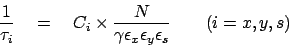
\includegraphics{img1.png}

\[
 \frac{1}{\tau_i} \quad = \quad C_i \times \frac{N}{\gamma \epsilon_x
   \epsilon_y \epsilon_s} \qquad (i = x, y, s) 
\]

where C$_i$ accounts for some constants and the integrals for the
scattering functions, N is the number of particles in the bunch,
$\gamma$ is the relativistic factor and $\epsilon_i$ are the normalized
emittances in the horizontal, vertical and longitudinal plane
respectively. It thus follows that the second required input is a
description of the beam parameters, which is achieved via the
``\textbf{beam}'' command (see below). 

Once the optical functions and the beam parameters have been defined,
the evaluation of the scattering growth times follows via the
``\textbf{ibs}'' command.  The ``\textbf{ibs}'' command should be
immediately preceded by a call of ``\textbf{twiss}''. In particular, the
``\textbf{emit}'' command should be followed by another call of
``\textbf{twiss}'' before ``\textbf{ibs}'' is used.      

If ``\textbf{twiss}'' calculates the optical functions at the end of
each element ``\textbf{ibs}'' performs a linear extrapolation to
determine their values  at the center of the elements. If
``\textbf{twiss}'' already computes the optical functions at the center
of each element ``\textbf{ibs}'' uses these  values directly without
making any interpolation.   

The logical follow-up of the MAD-X commands is illustrated in the two
examples provided with the IBS-module. 
  
\section{Input of the beam parameters}
This section briefly describes the parameters which have to be present
in the  ``\textbf{beam}'' command in order to run the IBS-module:  

\subsection{Particle type}
The parameter ``\textbf{particle=}'' is mandatory. It can take one of
the following \textbf{three} values: \textbf{proton, electron or
  ion}. For proton and electron, the parameter ``particle'' is the only
one to be defined. In case \textbf{ion} is used, two additional
parameters have to be defined, namely ``\textbf{mass=}'', which is
typically the number of nucleons for the corresponding ion multiplied by
\textbf{nmass} the unified atomic mass unit [0.931494013 GeV/(c**2)] ,
and ``\textbf{charge=}'' for the number of charges.   

\subsection{Energy}
The definition of the energy (total, kinetic, total energy of the ions
or energy per nucleon) is a difficult one. In the present approach, the
energy is the \textbf{total} energy of the particle. For ions, the
expected input is the \textbf{proton equivalent} energy, i.e. the total
energy a proton would have when circulating in the defined machine. As
an illustration, in the LHC, protons will be injected with an energy of
450 GeV. Consequently, to evaluate the growth times for Lead ions at
injection in the LHC, one has to input
\textbf{energy=450*charge}. Therefore the above example of Lead at the
LHC injection energy may look as follows in the MAD-X input language:  

\begin{verbatim}
nucleon = 208; 
charge = 82; 
beam, particle = ion, charge = charge,
      energy = 450*charge, mass = nucleon*nmass;  
\end{verbatim}

An important check for the correctness of the input is the printed value
of the relativistic factor  $\gamma$. The latter should correspond to:   

%  MATH
%  \begin{displaymath}
% \gamma_{ion} \quad = \quad \gamma_{proton} \times \frac{charge}{nucleon}
% \end{displaymath}
%  
%%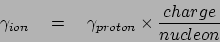
\includegraphics{img5.png}

\[
\gamma_{ion} \quad = \quad \gamma_{proton} \times \frac{charge}{nucleon}
\]

\subsection{Number of particles}
The number of particles (or number of ions) is defined with the
parameter ``\textbf{npart=}''.  

\subsection{Beam sizes - Emittances}
This part of the input is used to define the normalized emittances
(horizontal, vertical and longitudinal). The required parameters are the
\textbf{physical} transverse emittances (\textbf{ex=} and \textbf{ey=}
[$\pi$ m]), the longitudinal emittance (\textbf{ET=}) which is
defined    as the product of the bunch length (\textbf{sigt=}
[m]) and the relative energy spread (\textbf{sige=}). If only
the longitudinal emittance is defined (and not the \textbf{sigt}
and \textbf{sige} as well), an RF cavity is also
necessary. Otherwise, the bunch length (\textbf{sigt}) and the
relative energy spread (\textbf{sige}) should also be defined.   

\subsection{File Attribute}
If FILE="file\_name" appears MAD-X produces a table and writes on a file
for each element of the machine: ELEMENT NAME, Position S [m], DELS [m]
(Length Difference of consecutive Elements in the Table),  TLI
(Longitudinal growth time), TXI (Horizontal growth time), TYI (Vertical
growth time), BETX [m], ALFX [1], DX [m], DPX [1], BETY [m], ALFY [1],
DY [m], DPY [1].  

\subsection{Features}
The average growth rates in [sec] are defined as variables called
ibs.tx, ibs.ty, ibs.tl for the horizontal, vertical and longitudinal
growth times respectively. One can access them simply by calling them
after the ibs commant is called.   

 Example: 
\begin{verbatim} 
ibs; 
Tx = ibs.tx; 
\end{verbatim}
   
This defines a variable Tx which is the average horizontal growth rate in seconds. 

\section{Examples}
The two examples provided for the module Intra-Beam Scattering
illustrate the commands required to run the module. The two examples
have been selected such as to highlight the differences between a
computation for protons and that for ions. Both examples compute the IBS
growth times at injection into the LHC. The examples are located
\href{http://cern.ch/madx/madx.old}{here}.  


% Frank Schmidt 2003-05-23 
